\documentclass{article}

\usepackage[english]{babel}
\usepackage[letterpaper,top=2cm,bottom=2cm,left=3cm,right=3cm,marginparwidth=1.75cm]{geometry}
\usepackage[T1]{fontenc}
\usepackage[utf8]{inputenc}
\usepackage{amsmath}
\usepackage{amssymb}
\usepackage{booktabs}
\usepackage{float}
\usepackage{graphicx}
\usepackage{cite}
\usepackage[colorlinks=true, allcolors=blue]{hyperref}
\usepackage{microtype}
\usepackage{authblk}
\usepackage{tabularx}
\usepackage{subfigure}
\usepackage[table]{xcolor}
\usepackage{longtable}

\setlength{\parskip}{1.5em}
\linespread{1.2}

\providecommand{\keywords}[1]
{
  \small
  \textbf{\textit{Keywords---}} #1
}

\title{Beyond Euclidean Space: Geometric Alignment for Structure-Aware Dense Retrieval}
\author{}
\date{}

\begin{document}
\maketitle


\begin{abstract}
Retrieving structured documents requires understanding both their content and how that content is organized. This study explores whether hyperbolic representations can help SANTA learn these relationships and improve dense retrieval. We focus on its Structured Data Alignment (SDA) component, which aligns structured data with natural-language text, and consider two hyperbolic representations: the Poincar\'e ball and the Lorentz hyperboloid. We plan to evaluate these variants on CodeSearchNet and Adv for code retrieval, alongside an S1000D XML retrieval dataset to be constructed for this study. Comparisons with the original SANTA model will use consistent encoder and training settings. The evaluation will examine retrieval effectiveness across the three datasets and hierarchical relationship preservation in S1000D XML. Our aim is to understand when geometric alignment helps retrieve structured technical documents and whether better retrieval is accompanied by better preservation of their structure.
\end{abstract}

\keywords{Dense retrieval; Hyperbolic representation learning; Geometric alignment; S1000D XML}


\newpage

\section{Introduction}
\label{sec:01_introduction}

\subsection{Research Background and Motivation}
Structure-aware pretraining can improve dense retrieval over structured data by aligning structured content with natural-language text and learning structural semantics, as demonstrated by SANTA in code and product search~\cite{li2023structure}.
From a geometric perspective, Poincar\'e embeddings provide a means of jointly representing hierarchy and similarity in hyperbolic space, offering a compact representation of data with latent hierarchical structure~\cite{nickel2017poincare}.
% Explain why semantic similarity alone may not preserve the structure relevant to retrieval.

\subsection{Research Gap and Objectives}
Hyperbolic geometry provides a framework for representing hierarchical relationships through models such as the Poincar\'e ball and the Lorentz hyperboloid~\cite{nickel2018learning}. An important development in machine learning was the work of Nickel and Kiela~\cite{nickel2017poincare}, who demonstrated that Poincar\'e embeddings could capture hierarchy and similarity in low-dimensional representations, with favorable results on taxonomy reconstruction and link prediction. These findings suggest that representation geometry can support the learning of hierarchical structure. More recently, HypRAG applied Lorentz-based representations to dense retrieval for retrieval-augmented generation, using geometry-aware pooling to preserve hierarchical information when aggregating token representations into document embeddings~\cite{madhu2026hyprag}. Its evaluations on MTEB and RAGBench reported improvements over the evaluated Euclidean baselines in embedding quality and in context and answer relevance, providing evidence for the practical value of hyperbolic representations in retrieval settings. For structure-aware dense retrieval, this motivates examining how hyperbolic geometry can complement the alignment between structured data and natural-language descriptions. Specifically, this study aims to incorporate hyperbolic representations into the Structured Data Alignment (SDA) component of SANTA~\cite{li2023structure} and evaluate whether this geometric choice improves retrieval performance compared with its original formulation.

\subsection{Contributions}
% Revise the evaluation claims against the completed experiments.
In this study, we propose H-SANTA, a hyperbolic extension of SANTA, to investigate whether geometric alignment can better preserve structural relationships and improve dense retrieval. Motivated by the capacity of hyperbolic geometry to represent hierarchies, H-SANTA incorporates hyperbolic representations into SDA to align structured content with natural-language text. Our objective is to assess both retrieval effectiveness and structural preservation, rather than infer structural learning from retrieval gains alone. The main contributions are as follows:
\begin{enumerate}
    \item We propose H-SANTA, which explores Poincar\'e ball and Lorentz hyperboloid representations within SANTA's SDA component for structure-aware dense retrieval.
    \item We plan to construct an S1000D XML retrieval dataset and evaluate H-SANTA against the original SANTA on CodeSearchNet, Adv, and S1000D, examining retrieval effectiveness across datasets and hierarchical structure preservation in S1000D.
\end{enumerate}

\newpage

\section{Related Work}
\label{sec:02_related_work}

\subsection{Dense Retrieval}
Dense retrieval represents queries and documents as dense vectors and ranks documents through learned similarity functions. DPR~\cite{karpukhin2020dense} established a widely used dual-encoder formulation, learning query and passage representations from supervised question--passage pairs. Subsequent research improved both training and representation granularity: ANCE~\cite{xiong2021approximate} mined challenging negatives from a dynamically updated corpus index, while ColBERT~\cite{khattab2020colbert} retained token-level representations and computed fine-grained matching through late interaction. Retrieval-oriented pretraining also became an important direction. For example, coCondenser~\cite{gao2022unsupervised} introduced a corpus-level contrastive objective to prepare the passage embedding space before supervised training. Together, these approaches show that retrieval performance depends on the representation architecture, negative sampling, and pretraining objectives, providing essential controls when evaluating changes to representation geometry.

More recent research has expanded toward zero-shot retrieval and general-purpose embeddings built from large language models (LLMs). HyDE~\cite{gao2023precise} generated hypothetical documents from queries and encoded them to retrieve real documents without task-specific relevance labels. Wang et al.~\cite{wang2024improving} used LLM-generated synthetic data to train text embeddings through contrastive learning, evaluating generalization on BEIR and MTEB. The Qwen3 Embedding technical report~\cite{zhang2025qwen3} further combined foundation models, synthetic data, and multi-stage training for multilingual text embedding and retrieval. These developments broaden the available retrieval backbones and training resources, while motivating evaluation beyond a single domain. For structured content, SANTA~\cite{li2023structure} introduced Structured Data Alignment and Masked Entity Prediction, demonstrating their effectiveness in code and product search. Building on this direction, the present study examines whether hyperbolic alignment within SDA improves S1000D XML retrieval and preserves relevant hierarchical relationships, with encoder and training conditions controlled to distinguish geometric effects from other sources of improvement.

\subsection{Hyperbolic Representation Learning}
The use of hyperbolic geometry to represent relational structure predates modern neural embedding methods. Krioukov et al.~\cite{krioukov2010hyperbolic} connected negative curvature with degree heterogeneity and clustering in complex networks, providing a basis for relating geometry to structural organization. In 2017, Nickel and Kiela~\cite{nickel2017poincare} introduced Poincar\'e embeddings for learning hierarchy and similarity jointly. On the WordNet noun hierarchy, they compared Poincar\'e, Euclidean, and translational embeddings across dimensions using reconstruction and held-out link prediction, with mean rank and mean average precision showing strong low-dimensional performance. Their 2018 study~\cite{nickel2018learning} investigated Lorentz-based optimization on WordNet, EuroVoc, ACM, and MeSH, evaluating relation ranking and correlations between embedding norms and taxonomic depth. Its improvements concerned the learned embeddings and optimization procedure; the Poincar\'e and Lorentz models describe the same hyperbolic geometry at matching dimension and curvature. Also in 2018, Ganea et al.~\cite{ganea2018hyperbolic} extended hyperbolic learning to classifiers and neural layers. Comparisons on binary SNLI entailment and synthetic noisy-prefix recognition showed clearer advantages for more tree-like prefix relationships, while SNLI results were broadly comparable to Euclidean counterparts.

Subsequent applications examined how these geometric properties interact with task objectives and model components. Hyper-Know~\cite{ma2021knowledge} combined Poincar\'e representations, knowledge-graph attention, and adaptive regularization for recommendation. On Amazon-book, Last-FM, and Yelp2018, held-out interaction ranking and component ablations assessed Recall@K and NDCG@K, reporting improvements over the evaluated baselines. These results support the combined approach, rather than attributing all gains to geometry alone. Weber et al.~\cite{weber2024flattening} trained segmentation models on Cityscapes and tested them on five additional driving datasets, comparing hierarchical, flat Euclidean, and hyperbolic classifiers. Flat Euclidean models remained strong accuracy baselines, whereas hyperbolic representations showed particular benefits for parent-level calibration under domain shift. More directly related to retrieval, HypRAG~\cite{madhu2026hyprag} evaluated Lorentz-based text encoders on MTEB and RAGBench, comparing embedding quality and generated-answer grounding and relevance. Pooling ablations and analyses of radial separation between general and specific concepts examined how document aggregation retained hierarchical information. Together, these studies motivate evaluating the modified SANTA model on S1000D XML retrieval through controlled comparisons of geometry and alignment components, alongside direct checks of the structural relationships retained by its representations. Retrieval gains alone would not establish successful structural learning.


\newpage

\section{Preliminary}
\label{sec:03_problem_formulation}

\subsection{SANTA and Structured Data Alignment}
SANTA learns representations of natural-language text and structured data in a shared embedding space~\cite{li2023structure}. Its Structured Data Alignment (SDA) objective uses paired structured and unstructured content as positive examples and contrastively distinguishes matched pairs from mismatched examples. Masked Entity Prediction provides complementary supervision by reconstructing masked entities in structured data. These existing objectives provide the background for examining the geometry of SDA; the proposed changes to its representations and alignment objective are described in Section~\ref{sec:04_method}.

\subsection{Hyperbolic Geometry for Representation Learning}
Hyperbolic space has constant negative sectional curvature and supports compact representations of hierarchical relationships~\cite{nickel2017poincare,nickel2018learning}. Let $c>0$ denote the magnitude of curvature, so that the curvature is $-c$, and let $d$ denote the intrinsic dimension. The Poincar\'e ball and Lorentz hyperboloid are two coordinate models of this same geometry. Their definitions below use a common curvature convention to support subsequent comparisons.

\subsubsection{Poincar\'e Ball Model}
The Poincar\'e ball is defined by
\begin{equation}
 \mathbb{B}_c^d=\{\mathbf{x}\in\mathbb{R}^d:c\|\mathbf{x}\|_2^2<1\},
 \qquad g_{\mathbf{x}}=(\lambda_{\mathbf{x}}^c)^2 I_d,
 \qquad \lambda_{\mathbf{x}}^c=\frac{2}{1-c\|\mathbf{x}\|_2^2}.
 \label{eq:poincare-domain}
\end{equation}
Its geodesic distance is
\begin{equation}
 d_{\mathbb B}^c(\mathbf{x},\mathbf{y})=
 \frac{1}{\sqrt c}\operatorname{arcosh}\!\left(
 1+\frac{2c\|\mathbf{x}-\mathbf{y}\|_2^2}
 {(1-c\|\mathbf{x}\|_2^2)(1-c\|\mathbf{y}\|_2^2)}\right).
 \label{eq:poincare-distance}
\end{equation}
A tangent vector $\mathbf{v}\in T_{\mathbf{0}}\mathbb{B}_c^d\cong\mathbb{R}^d$ can be mapped into the ball using the exponential map~\cite{ganea2018hyperbolic}:
\begin{equation}
 \exp_{\mathbf{0}}^{\mathbb B,c}(\mathbf{v})=
 \tanh(\sqrt c\|\mathbf{v}\|_2)
 \frac{\mathbf{v}}{\sqrt c\|\mathbf{v}\|_2}.
 \label{eq:poincare-exp}
\end{equation}
At $\mathbf{v}=\mathbf{0}$, the map is defined by continuity as $\mathbf{0}$. The conformal factor makes distances grow near the boundary, allowing radial position to encode hierarchical depth when supported by the learning objective.

\subsubsection{Lorentz Hyperboloid Model}
For $\mathbf{x}=(x_0,\mathbf{x}_s)$ and $\mathbf{y}=(y_0,\mathbf{y}_s)$ in $\mathbb{R}^{d+1}$, define the Lorentz inner product and upper hyperboloid by
\begin{equation}
 \langle\mathbf{x},\mathbf{y}\rangle_L=-x_0y_0+\mathbf{x}_s^\top\mathbf{y}_s,
 \qquad
 \mathbb{H}_c^d=\{\mathbf{x}:\langle\mathbf{x},\mathbf{x}\rangle_L=-1/c,\ x_0>0\}.
 \label{eq:lorentz-domain}
\end{equation}
The induced metric on its tangent spaces is positive definite, and the geodesic distance is~\cite{nickel2018learning}
\begin{equation}
 d_{\mathbb H}^c(\mathbf{x},\mathbf{y})=
 \frac{1}{\sqrt c}\operatorname{arcosh}(-c\langle\mathbf{x},\mathbf{y}\rangle_L).
 \label{eq:lorentz-distance}
\end{equation}
At the origin $\mathbf{o}=(1/\sqrt c,\mathbf{0})$, a tangent vector has the form $\mathbf{v}=(0,\mathbf{h})$. Its exponential map is
\begin{equation}
 \exp_{\mathbf{o}}^{\mathbb H,c}(0,\mathbf{h})=
 \left(\frac{\cosh(\sqrt c\|\mathbf{h}\|_2)}{\sqrt c},
 \frac{\sinh(\sqrt c\|\mathbf{h}\|_2)}{\sqrt c\|\mathbf{h}\|_2}\mathbf{h}\right),
 \label{eq:lorentz-exp}
\end{equation}
with value $\mathbf{o}$ at $\mathbf{h}=\mathbf{0}$. This construction produces a valid manifold point from a Euclidean encoder representation interpreted as a tangent vector.

\subsubsection{Correspondence Between the Models}
The distance-preserving coordinate transformation from the ball to the hyperboloid and its inverse are
\begin{equation}
 \Phi_c(\mathbf{z})=
 \left(\frac{1+c\|\mathbf{z}\|_2^2}{\sqrt c(1-c\|\mathbf{z}\|_2^2)},
 \frac{2\mathbf{z}}{1-c\|\mathbf{z}\|_2^2}\right),
 \qquad
 \Phi_c^{-1}(\mathbf{x})=\frac{\mathbf{x}_s}{\sqrt c x_0+1}.
 \label{eq:hyperbolic-correspondence}
\end{equation}
Consequently, $d_{\mathbb H}^c(\Phi_c(\mathbf{z}),\Phi_c(\mathbf{w}))=d_{\mathbb B}^c(\mathbf{z},\mathbf{w})$. The origin metrics have different coordinate scales: matched tangent vectors satisfy $\mathbf{h}=2\mathbf{v}$ in Eqs.~\ref{eq:poincare-exp} and~\ref{eq:lorentz-exp}. Comparisons should therefore control intrinsic dimension, curvature, and representation scale; differences between implementations may reflect optimization or numerical behavior rather than different underlying geometries. These definitions supply the distances and mappings needed to formulate hyperbolic SDA, while its scoring function and training objective belong to the proposed method.

\newpage

\section{Proposed Method}
\label{sec:04_method}

\subsection{Architecture}
\begin{figure}[htbp]
    \centering
    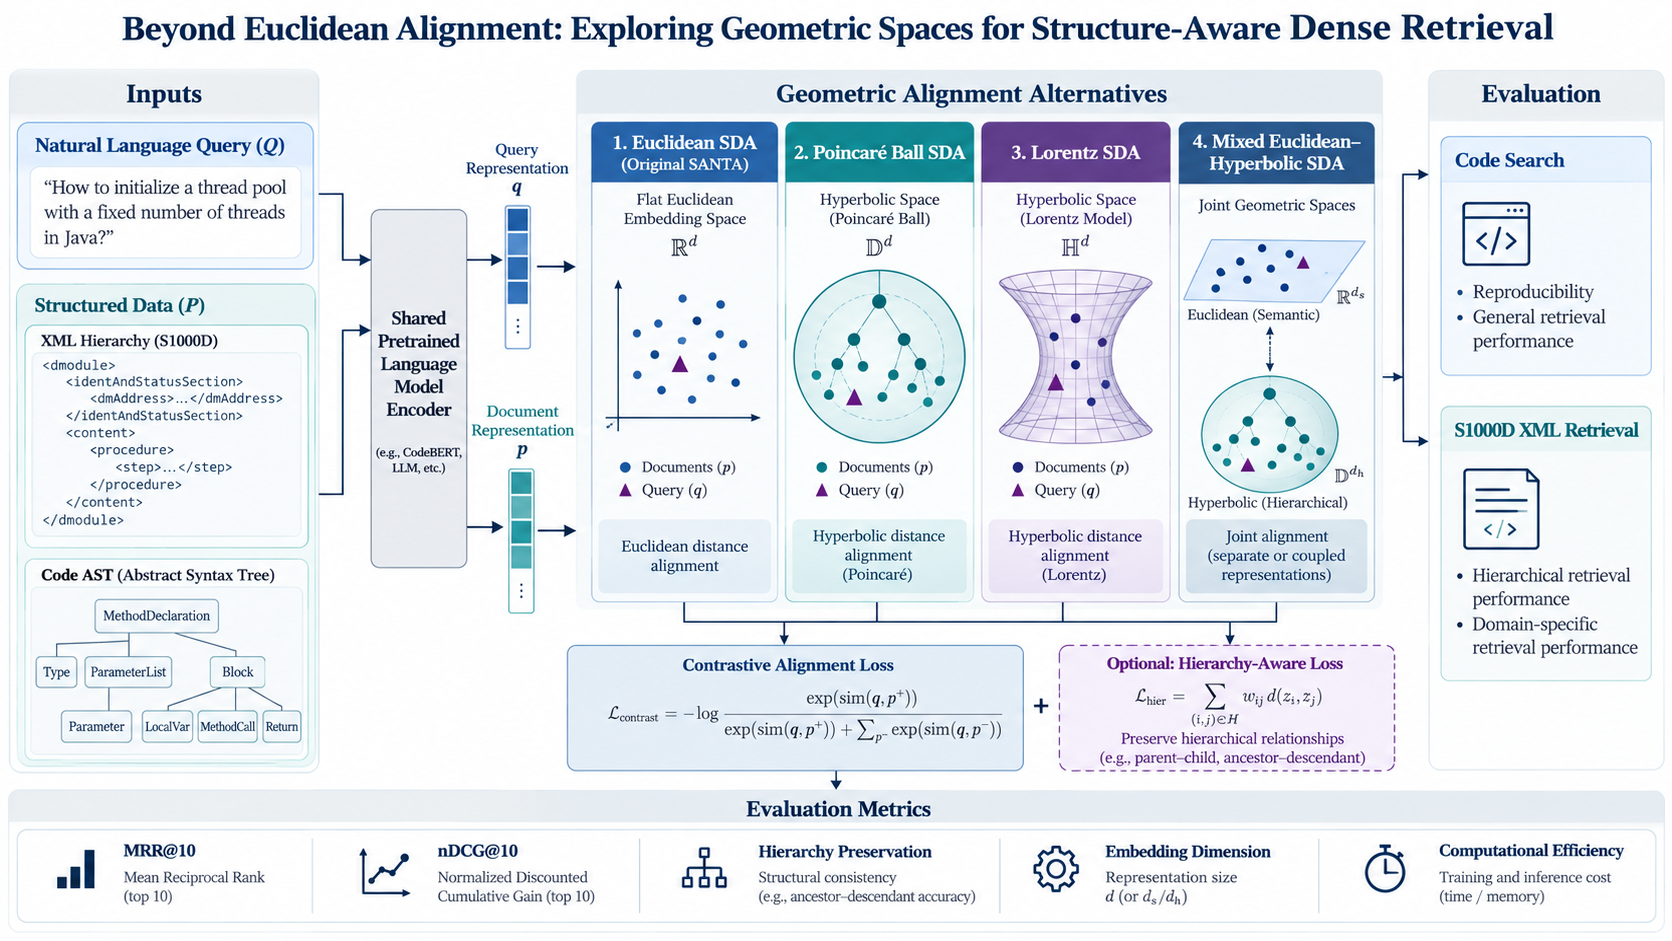
\includegraphics[width=\textwidth]{images/overview_ai.png}
    \caption{Conceptual architecture of geometric alignment for structure-aware dense retrieval. The diagram summarizes candidate alignment geometries and evaluation settings; the mixed-geometry branch and hierarchy-aware objective represent optional extensions.}
    \label{fig:architecture}
\end{figure}
% Refine the architecture description once the alignment variants are finalized.

\subsection{Structure-Aware Representations}
% Describe how semantic and structural information enter the representations.

\subsection{Geometric Alignment}
% Define the alignment mechanism and its mathematical assumptions.

\subsection{Learning Objectives and Optimization}
% Specify losses, supervision, optimization, and safeguards against information leakage.

\subsection{Retrieval Procedure}
% Describe query encoding, document indexing, scoring, and ranking at inference.


\newpage

\section{Experimental Setup}
\label{sec:05_experimental_setup}

\subsection{Research Questions}
% Specify testable questions about retrieval effectiveness, structural behavior, and efficiency.

\subsection{Datasets and Data Preparation}
% Document dataset provenance, structure annotations, splits, and preprocessing.

\subsection{Baseline Methods}
% Specify comparable baselines and ensure fair backbone, supervision, and tuning conditions.

\subsection{Evaluation Metrics and Statistical Analysis}
% Define retrieval and structural metrics, uncertainty estimates, and appropriate comparisons.

\subsection{Implementation Details}
% Report hyperparameters, hardware, random seeds, tuning budgets, and reproducibility details.


\newpage

\section{Experimental Results and Analysis}
\label{sec:06_results}

\subsection{Retrieval Effectiveness}
% Compare original SANTA, Poincare SDA, and Lorentz SDA on CodeSearchNet, Adv, and S1000D.
% Follow the established evaluation protocols and report uncertainty across random seeds.
% Report measured results only; do not insert hypothetical findings.

\subsection{Hierarchical Structure Preservation}
% Evaluate parent--child and ancestor--descendant relationships in held-out S1000D data.
% Distinguish relational proximity from hierarchy direction and compare structural and retrieval outcomes.

\subsection{Ablation Analysis}
% Isolate geometric alignment effects while controlling encoders, supervision, negative samples, and training budgets.
% Examine curvature and intrinsic dimension with consistent representation scales and validation-based tuning.

\subsection{Case Study}
% Compare representative successes and failures, showing retrieved content and its position in the XML hierarchy.
% Explain whether observed errors concern semantic relevance, structural relationships, or both.

\newpage

\section{Discussion}
\label{sec:07_discussion}

\subsection{Interpretation of Findings}
% Answer the research questions and relate findings to prior work.

\subsection{Implications for Structure-Aware Retrieval}
% Explain when geometric alignment is useful and the conditions limiting its value.

\subsection{Limitations and Threats to Validity}
% Discuss data, structural assumptions, generalizability, and experimental confounds.


\newpage

\section{Conclusion}
\label{sec:08_conclusion}

% Summarize supported contributions and findings, then identify future work.


\bibliographystyle{IEEEtran}
\bibliography{custom}

\appendix
\newpage

\section{Supplementary Method and Experimental Details}
\label{sec:appendix}

% Add derivations, complete configurations, and supplementary results as needed.


\end{document}
